\section{Results}\label{sec:results}
\todo{Results are filled in as experiments complete; tables below define the planned layout.}

\subsection{Each action controls what it should}
We first examine \method{} at size S (60k steps). On 512 validation windows, futures generated from the actions inferred from the real clip have a latent error of \val{use/S_arms/replay}. Replacing every arm's action with that of another window raises the error by \val{use/S_arms/swap}\,\% (\val{use/S_arms/swap_in}\,\% inside the arm regions, \val{use/S_arms/swap_out}\,\% outside); replacing the endoscope action raises it by \val{use/S_arms/cam_swap}\,\% (\val{use/S_arms/cam_swap_in}\,\% inside, \val{use/S_arms/cam_swap_out}\,\% outside). The flow-matching loss at a high noise level ($\tau=0.9$) separates the two more sharply: another window's arm actions raise it by \val{use/S_arms/swap_t9_in}\,\% inside the arm regions and \val{use/S_arms/swap_t9_out}\,\% outside, and another window's endoscope action by \val{use/S_arms/cam_swap_t9_in}\,\% inside and \val{use/S_arms/cam_swap_t9_out}\,\% outside. With the arm actions zeroed, replacing the endoscope action still raises the error by \val{use/S_arms/cam_swap_zeroed}\,\%, so the learned actions have not absorbed the endoscope motion. Of the 8 dimensions of each arm action, \val{use/S_arms/active} are active, their posterior mean varying across windows with a variance above 0.01 (KL \val{use/S_arms/kl}\,nats per arm).

Fig.~\ref{fig:horizon} shows the fidelity over the horizon. On the \val{main/n_cases} test cases (\val{ctl/n_windows} windows), commanded endoscope motions are realised in the commanded direction in at least \val{ctl/S_arms/sign_min}\,\% of the windows for each of the six commands (pan, tilt and zoom, both ways), at a median \val{ctl/S_arms/gain_range}\,\% of the commanded magnitude. Replacing one arm's action changes the generated video mainly where that arm's instrument is: its region receives \val{ctl/S_arms/share}\,\% of the change while covering \val{ctl/S_arms/area}\,\% of the frame (median ratio \val{ctl/S_arms/locality}). On generated frames, the instrument detector recovers the instruments of the real future with precision \val{ctl/S_arms/ecs_p} and recall \val{ctl/S_arms/ecs_r}; \val{ctl/S_arms/halluc}\,\% of the generated instruments are not mounted according to the robot log, against \val{ctl/reference/real_halluc}\,\% when the detector is applied to the real frames or their VAE reconstructions, and \val{ctl/S_none/halluc}\,\% without actions.

\begin{figure}[t]
\centering
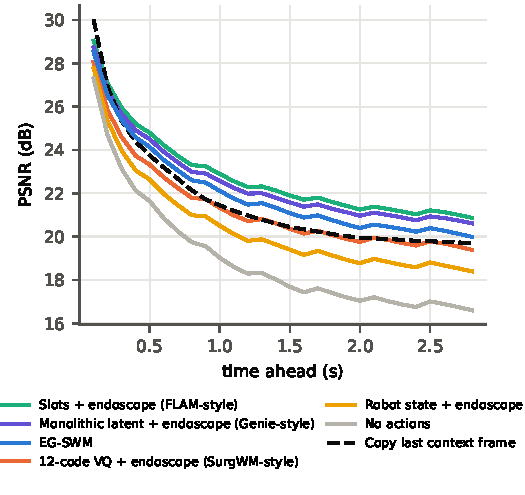
\includegraphics[width=\columnwidth]{e1_horizon.pdf}
\caption{PSNR of each predicted frame, 0.1--2.8\,s after the last context frame (mean over the \val{main/n_windows} test windows).}
\label{fig:horizon}
\end{figure}

\subsection{Fidelity}
Table~\ref{tab:main} compares the interfaces on \val{main/n_windows} windows spread evenly over the test cases. Paired over the same windows, \method{} improves on copying the last context frame by \val{diff/S_arms-copy_last/psnr}\,dB PSNR (95\,\% case-bootstrap interval \val{diff/S_arms-copy_last/psnr_ci}, \val{diff/S_arms-copy_last/wins} of \val{main/n_cases} cases) and \val{diff/S_arms-copy_last/ssim} SSIM, but is \val{diff/S_arms-copy_last/lpips} LPIPS worse: it trails the copied frame in the first \val{horizon/trail}\,s and leads by \val{horizon/lead}\,dB from 0.5\,s to the end of the 2.8\,s horizon. Replaying the inferred actions is worth \val{main/S_arms/delta_psnr}\,dB over the actions of another window, and the same model trained without actions is \val{diff/S_arms-S_none/psnr}\,dB \val{diff/S_arms-S_none/psnr_ci} worse, in \val{diff/S_arms-S_none/wins} of \val{main/n_cases} cases.

\subsection{Fidelity and control pull apart}
The interfaces whose learned action covers the whole frame give the best fidelity (Table~\ref{tab:main}): slot actions improve on \method{} by \val{diff/S_slots-S_arms/psnr}\,dB PSNR \val{diff/S_slots-S_arms/psnr_ci} (in \val{diff/S_slots-S_arms/wins} of the \val{main/n_cases} test cases) and the monolithic latent action by \val{diff/S_global-S_arms/psnr}\,dB \val{diff/S_global-S_arms/psnr_ci} (\val{diff/S_global-S_arms/wins} of \val{main/n_cases}), and adding a scene action, pooled outside every arm region, to \method{} improves \val{diff/S_arms_scene-S_arms/wins} of \val{main/n_cases} cases by \val{diff/S_arms_scene-S_arms/psnr}\,dB \val{diff/S_arms_scene-S_arms/psnr_ci} while making the arm actions more local (ratio \val{ctl/S_arms_scene/locality}) and lowering hallucinations to \val{ctl/S_arms_scene/halluc}\,\%. All three take over the endoscope: with the learned actions zeroed, a commanded endoscope motion is realised at \val{ctl/S_slots/gain_range}\,\% of its magnitude with slots, \val{ctl/S_global/gain_range}\,\% with the monolithic action and \val{ctl/S_arms_scene/gain_range}\,\% with the scene action, against \val{ctl/S_arms/gain_range}\,\% for \method{}. On the validation windows, another clip's endoscope action raises the replay error of the slot model by only \val{use/S_slots/cam_swap}\,\% (\method{}: \val{use/S_arms/cam_swap}\,\%), and the monolithic model is as faithful without an endoscope action as with it (difference \val{diff/S_global_nocam-S_global/psnr}\,dB \val{diff/S_global_nocam-S_global/psnr_ci}). At $\tau=0.9$, another clip's slot or monolithic action raises the flow-matching loss as much outside the arm regions as inside (slots +\val{use/S_slots/swap_t9_out}\,\% and +\val{use/S_slots/swap_t9_in}\,\%, monolithic +\val{use/S_global/swap_t9_out}\,\% and +\val{use/S_global/swap_t9_in}\,\%; \method{}'s arm actions +\val{use/S_arms/swap_t9_out}\,\% and +\val{use/S_arms/swap_t9_in}\,\%), so these actions steer no particular instrument. In a 12k-step pilot, the scene action carried as much endoscope motion when it was inferred from latents aligned by the measured endoscope motion, so it does not simply copy the motion it sees. We hypothesise that it describes content the context cannot predict, such as tissue entering the field of view, whose position reveals the motion; this remains to be tested directly. Under action replay, an action inferred from the real future can carry how that future looks, and the more of the frame it covers, the more it carries.

Among the interfaces that keep the endoscope controllable, \method{} is the most faithful by a wide margin: it leads the 12-code VQ action of SurgWM~\cite{surgwm} by \val{diff/S_arms-S_global_vq/psnr}\,dB \val{diff/S_arms-S_global_vq/psnr_ci} (in \val{diff/S_arms-S_global_vq/wins} of \val{main/n_cases} cases) and robot-state tokens with the endoscope action by \val{diff/S_arms-S_state/psnr}\,dB \val{diff/S_arms-S_state/psnr_ci} (\val{diff/S_arms-S_state/wins} of \val{main/n_cases}). The VQ action carries little (another clip's code raises the replay error by \val{use/S_global_vq/swap}\,\%), and its model falls below the copied frame (\val{diff/S_global_vq-copy_last/psnr}\,dB \val{diff/S_global_vq-copy_last/psnr_ci}). \method{} is thus the only interface that steers each instrument and the endoscope and still improves on the copied frame. Since none of the frame-wide actions has a physical controller that could set it in a simulation, \method{} keeps every learned action bound to an arm.

The gap in fidelity is concentrated where the arm actions cannot act (Table~\ref{tab:binding}). A mounted instrument has an image region in \val{bind/steps}\,\% of the latent steps of the test windows; \val{bind/none}\,\% of the mounted instruments have none in their window, being out of view, occluded, missed by the detector or not matched to the robot log, and \val{bind/some}\,\% have one in some steps only. In the \val{bind/n/two} test windows (of \val{main/n_windows}) in which at least two mounted instruments are bound for most of the horizon, \method{} trails the monolithic latent by \val{bind/two/S_global-S_arms}\,dB and the slots by \val{bind/two/S_slots-S_arms}\,dB. In the \val{bind/n/none} windows in which none is bound, it trails them by \val{bind/none/S_global-S_arms} and \val{bind/none/S_slots-S_arms}\,dB and falls below the copied frame. The frame-wide actions do not depend on the binding and describe whatever moves instead, so a higher binding coverage could narrow the gap without a frame-wide action.

\begin{table}[t]
\centering
\caption{PSNR on the \val{main/n_windows} test windows grouped by how many mounted instruments are bound to an arm region for most of the predicted steps.}
\label{tab:binding}
\resizebox{\columnwidth}{!}{\begin{tabular}{lccc}
\toprule
 & \multicolumn{3}{c}{Instruments bound (windows)} \\
\cmidrule(lr){2-4}
Model & none (93) & one (179) & $\geq$2 (728) \\
\midrule
Copy last context frame & 23.79 & 20.68 & 21.54 \\
None (unconditional) & 20.27 & 18.08 & 19.01 \\
Robot state & 20.63 & 18.28 & 19.37 \\
Robot state + camera & 22.36 & 19.53 & 20.42 \\
Monolithic latent (Genie) & 24.97 & 21.59 & 22.39 \\
Monolithic latent + camera & 25.10 & 21.58 & 22.35 \\
Monolithic VQ + camera (SurgWM-style) & 23.73 & 20.36 & 21.23 \\
Slots + camera (FLAM-style) & 25.32 & 21.85 & 22.67 \\
EG-SWM, no camera action & 20.11 & 20.42 & 21.96 \\
EG-SWM & 22.94 & 20.83 & 22.17 \\
EG-SWM + scene action & 24.56 & 21.27 & 22.37 \\
\bottomrule
\end{tabular}
}
\end{table}

\subsection{What each part of \method{} adds}\label{sec:parts}
The endoscope action is worth \val{diff/S_arms-S_arms_nocam/psnr}\,dB \val{diff/S_arms-S_arms_nocam/psnr_ci} to \method{}, in \val{diff/S_arms-S_arms_nocam/wins} of \val{main/n_cases} cases. Without it, the arm actions take on part of the frame-wide motion (at $\tau=0.9$, another clip's arm actions raise the loss outside the arm regions by \val{use/S_arms_nocam/swap_t9_out}\,\% instead of \val{use/S_arms/swap_t9_out}\,\%) and become less local (ratio \val{ctl/S_arms_nocam/locality} instead of \val{ctl/S_arms/locality}). Learned arm actions are worth \val{diff/S_arms_nocam-S_state_nocam/psnr}\,dB \val{diff/S_arms_nocam-S_state_nocam/psnr_ci} over robot-state tokens, both without the endoscope action. The state tokens alone add \val{diff/S_state_nocam-S_none/psnr}\,dB \val{diff/S_state_nocam-S_none/psnr_ci} over unconditional prediction and lower hallucinations from \val{ctl/S_none/halluc}\,\% to \val{ctl/S_state_nocam/halluc}\,\%; with them, the endoscope action is worth \val{diff/S_state-S_state_nocam/psnr}\,dB \val{diff/S_state-S_state_nocam/psnr_ci} and is realised at \val{ctl/S_state/gain_range}\,\% of its magnitude.

Grounding is what makes the arm actions local. When each arm's inverse-dynamics head and its input to the forward decoder cover the whole frame instead of the arm's instrument region, with one action per arm still bound through the robot log, fidelity barely changes (\val{diff/S_arms_poolglobal-S_arms/psnr}\,dB \val{diff/S_arms_poolglobal-S_arms/psnr_ci} better than \method{}, which leads in \val{diff/S_arms_poolglobal-S_arms/losses} of \val{main/n_cases} cases), but the locality ratio falls from \val{ctl/S_arms/locality} to \val{ctl/S_arms_poolglobal/locality}, \val{derived/pool_way}\,\% of the way to the monolithic action (\val{ctl/S_global/locality}), and the endoscope gain from \val{ctl/S_arms/gain} to \val{ctl/S_arms_poolglobal/gain}.

The forward decoder keeps the arm actions in use. Trained on the diffusion loss alone, only \val{use/S_arms_nofwd/active} of the 8 dimensions of each arm action stay active (KL \val{use/S_arms_nofwd/kl} instead of \val{use/S_arms/kl}\,nats per arm), another window's arm actions raise the replay error by \val{use/S_arms_nofwd/swap}\,\% instead of \val{use/S_arms/swap}\,\%, and replaying the inferred actions is worth \val{main/S_arms_nofwd/delta_psnr} instead of \val{main/S_arms/delta_psnr}\,dB over the actions of another window. The decoder improves fidelity by \val{diff/S_arms-S_arms_nofwd/psnr}\,dB PSNR \val{diff/S_arms-S_arms_nofwd/psnr_ci}, in \val{diff/S_arms-S_arms_nofwd/wins} of \val{main/n_cases} cases, and lowers FVD from \val{main/S_arms_nofwd/fvd} to \val{main/S_arms/fvd}, while the endoscope action is realised about as well without it (mean gain \val{ctl/S_arms_nofwd/gain} against \val{ctl/S_arms/gain}).

\begin{table*}[t]
\centering
\caption{Action-conditioned prediction on held-out SurgVU test cases (\val{main/n_cases} cases, 2.8\,s horizon, action replay, 50 Euler steps). PSNR, SSIM and LPIPS are means over cases with 95\,\% case-bootstrap intervals. Cam.\ gain: realised/commanded endoscope motion; Locality: share of the change inside the replaced arm's region over its area share; Halluc.: generated instruments not mounted per the robot log. \todo{ablation rows (whole-frame pooling, no forward decoder, wrong arm binding, console readout) as their runs finish}}
\label{tab:main}
\resizebox{\textwidth}{!}{\begin{tabular}{lcccccccc}
\toprule
Model & PSNR$\uparrow$ & SSIM$\uparrow$ & LPIPS$\downarrow$ & FVD$\downarrow$ & $\Delta$PSNR$\uparrow$ & Cam. gain$\uparrow$ & Locality$\uparrow$ & Halluc.$\downarrow$ \\
\midrule
Copy last context frame & 21.60\,{\scriptsize[20.94, 22.27]} & 0.681\,{\scriptsize[0.663, 0.699]} & 0.156\,{\scriptsize[0.145, 0.167]} & 653 & -- & -- & -- & -- \\
VAE reconstruction (ceiling) & 34.29\,{\scriptsize[33.97, 34.61]} & 0.949\,{\scriptsize[0.946, 0.952]} & 0.018\,{\scriptsize[0.017, 0.018]} & 22 & -- & -- & -- & 0.053 \\
Real frames (detector floor) & -- & -- & -- & -- & -- & -- & -- & 0.053 \\
None (unconditional) & 18.96\,{\scriptsize[18.49, 19.47]} & 0.583\,{\scriptsize[0.568, 0.599]} & 0.249\,{\scriptsize[0.238, 0.261]} & 422 & 0.00 & -- & -- & 0.130 \\
Robot state + camera & 20.44\,{\scriptsize[19.89, 21.01]} & 0.652\,{\scriptsize[0.636, 0.669]} & 0.206\,{\scriptsize[0.194, 0.218]} & 266 & 1.42 & 0.79 & -- & 0.078 \\
Monolithic latent + camera & 22.47\,{\scriptsize[21.94, 23.01]} & 0.703\,{\scriptsize[0.688, 0.718]} & 0.154\,{\scriptsize[0.145, 0.164]} & 180 & 3.17 & 0.16 & 1.46 & 0.074 \\
Monolithic VQ + camera (SurgWM-style) & 21.30\,{\scriptsize[20.76, 21.86]} & 0.671\,{\scriptsize[0.655, 0.687]} & 0.183\,{\scriptsize[0.172, 0.194]} & 206 & 2.11 & 0.81 & 1.53 & 0.082 \\
Slots + camera (FLAM-style) & 22.77\,{\scriptsize[22.24, 23.31]} & 0.713\,{\scriptsize[0.698, 0.727]} & 0.149\,{\scriptsize[0.139, 0.158]} & 169 & 3.55 & 0.05 & 1.44 & 0.078 \\
EG-SWM, no camera action & 21.52\,{\scriptsize[20.90, 22.15]} & 0.672\,{\scriptsize[0.654, 0.691]} & 0.176\,{\scriptsize[0.164, 0.189]} & 215 & 2.27 & -- & 2.02 & 0.080 \\
EG-SWM & 22.00\,{\scriptsize[21.43, 22.62]} & 0.691\,{\scriptsize[0.675, 0.708]} & 0.164\,{\scriptsize[0.153, 0.175]} & 186 & 2.78 & 0.70 & 2.42 & 0.076 \\
EG-SWM + scene action & 22.38\,{\scriptsize[21.82, 22.95]} & 0.701\,{\scriptsize[0.685, 0.717]} & 0.156\,{\scriptsize[0.146, 0.167]} & 174 & 3.04 & 0.22 & 3.50 & 0.072 \\
\bottomrule
\end{tabular}
}
\end{table*}
